\documentclass[sanserif]{beamer}
%\documentclass[sanserif,handout]{beamer}
\usepackage [T1] {fontenc} 
\usepackage{pdfpages}
\usepackage{citesupernumber}
\usepackage{multirow}
\usepackage{pgfpages}
%\pgfpagesuselayout{4 on 1}[letterpaper, landscape, border, shrink=5mm]
\usepackage{graphicx}
\usepackage{tikz}
\usetikzlibrary{shapes.geometric,fit,positioning}
\tikzset{
	semi/.style={
		semicircle,
		draw
	}
}

\hyphenpenalty=5000
\tolerance=1000


\definecolor{green}{rgb}{0.0,0.7,0.0}
\setbeamercolor{green}{fg=green}
\setbeamercolor{gray}{fg=gray} 
\setbeamercolor{red}{fg=red}
\setbeamercolor{black}{fg=black}
\setbeamercolor{white}{fg=white}
\definecolor{unf}{rgb}{0.0,0.2,0.9}
\definecolor{poz}{rgb}{0.7,0.7,0.0}
\definecolor{neg}{rgb}{0.7,0.0,0.0}
\setbeamercolor{unf}{fg=unf}
\setbeamercolor{poz}{fg=poz}
\setbeamercolor{neg}{fg=neg}


\setbeamerfont{italic}{shape=\slshape}
\setbeamerfont{upright}{shape=\upshape}
\setbeamerfont{tt}{family=\ttfamily}
\setbeamerfont{rm}{family=\sffamily}
\setbeamerfont{bold}{series=\bfseries}
\setbeamerfont{norm}{series=\normalfont}
\setbeamerfont{tiny}{size=\tiny}
\setbeamerfont{small}{size=\small}
\setbeamerfont{normal}{size=\normalsize}



\setbeamerfont{frametitle}{series=\bfseries}
\setbeamertemplate{bibliography item}[text]

\newcommand{\EQU}{\texttt{equals}}
\newcommand{\LogicNine}{\texttt{Logic-9}}
\newcommand{\EquOnly}{\texttt{equals only}}
\newcommand{\gray}[1]{ \usebeamercolor[fg]{gray}#1\usebeamercolor{normal text}}
\newcommand{\italics}[1]{\usebeamerfont{italic}#1\usebeamerfont{upright}}
\renewcommand{\tt}[1]{\usebeamerfont{tt}#1\usebeamerfont{rm}}
\newcommand{\bolds}[1]{\usebeamerfont{bold}#1\usebeamerfont{norm}}
\newcommand{\li}[1]{\begin{tabular}{p{0.01\textwidth} p{0.40\textwidth}}  $\bullet$ & \usebeamerfont{small} #1 \end{tabular}}

\setbeamertemplate{navigation symbols}{ \insertframenumber } 

\mode<presentation>
{
	\usetheme{Berkeley}
	\usecolortheme{orchid}
}

\title[Evolvability]{On the Evolution of\\Evolvability}
\author[]{Rosangela Canino-Koning}
\date{Wednesday 09 December 2015}

\begin{document}
\bibliographystyle{nature}

\frame{\titlepage}
%%%
% Hello everyone, thank's for coming
% Today, I'm going to talk about the evolution of evolvability


%%%%%%%%%%%%%%%%%% INTRODUCTION %%%%%%%%%%%%%%%%%%%
\section[Introduction]{Introduction}

\frame{
	\frametitle{What is Evolvability?}
	\begin{block}{Evolvability}
	"The potential of populations and genomes to produce adaptive variation and complex structures in response to mutation and selection."
	\end{block}

%%% 
% The idea of evolvability is tightly entwined with evolution. Evolvability is simply the potential to evolve. In itself, evolvability is not especially controversial. We have long known that different populations have different characteristics when it comes to their ability to respond to selection, or to adapt to environments. 
% But if there is variation in those features, is it possible that those features might themselves come under selection? Could Evolvability itself evolve?
% The idea that evolvability might evolve continues to be controversial, from the level at which such selection might occur, if there is selection at all, or rather if evolvability is a hitchiker. And where there is no controversy, there is confusion and disagreement, with a variety of definitions, measures, and features, down to the basics of what things help or hurt evolvability.
% In order to clear the air a bit, let's do a quick survey of how evolvability has been described and regarded over the years.

}

\subsection[Historical Context]{Historical Context}

\frame{
   \frametitle{Modern Synthesis - Heritability and Response to Selection\cite{fisher_genetical_1930,wright_evolution_1931,houle_comparing_1992}}
   
   	\begin{figure}[h!]
   		\begin{center}
   			\includegraphics[height=3.5cm]{pictures/Biologist_and_statistician_Ronald_Fisher.jpg}
   			\quad
   			\includegraphics[height=3.5cm]{pictures/Sewall_Wright.jpg}
   			\quad
   			\includegraphics[height=3.5cm]{pictures/2friendlydavid.jpg}
   			\caption{R. A. Fisher\cite{commons_english:_1957}, Sewall Wright\cite{_file:sewall_2012}, and David Houle\cite{houle_david_david_????}}
   		\end{center}
   	\end{figure}
%%%
% While evolvability, as such, was not specifically named until the late 80s, the idea of evolvability existed in the form of heritability, in the work of Fisher and Wright.
% Fisher's fundamental theorem of response to selection identifies narrow-sense heritability, or additive genetic variation, as the genetic component of population variation that accounted most for the response of a population to selection. Narrow-sense heritability is distinct from Broad-sense heritability, which includes effects from dominance and epistasis, which can confound the prediction of a population's response to selection.
% Later, in the work of Houle, we find a refinement to the idea of heritability, to use the coefficient of variation rather than narrow-sense heritability in order to predict response to selection.
% However you measure heritability, however, it lacks the ability to predict the effects of variation in genetic architecture on adaptation, or the effect of mutation. Something else is missing. 
}

\frame{
	\frametitle{Evolvability as a Distinct Concept - Evolvable Embryologies\cite{dawkins_13_2003,alberch_genes_1991}}
	
	   	\begin{figure}[h!]
	   		\begin{center}
	   			\includegraphics[height=5cm]{pictures/Richard_Dawkins_Cooper_Union_Shankbone.jpg}
	   			\qquad
	   			\includegraphics[height=5cm]{pictures/pere_alberch}
	   			\caption{Richard Dawkins\cite{shankbone_english:_2010} and Pere Alberch\cite{reiss_pere_2015}}
	   		\end{center}
	   	\end{figure}
	
%Beginning with Dawkins in 1989, and expanded by Alberch, we find the concept of Evolvability spelled out as an idea distinct from heritability. Both Dawkins and Alberch narrowly described variations in evolvability as being the result of "embryologies" or developmental processes that allow for greater complexity.
}


\frame{
	\frametitle{Expanding on Evolvability - Variation vs Variability%\cite{wagner_perspective_1996} FIGURE THIS OUT
		}
	   	\begin{figure}[h!]
	   		\begin{center}
	   			\includegraphics[height=5cm]{pictures/GPWOslo08_007_1.jpg}
	   			\qquad
	   			\includegraphics[height=5cm]{pictures/LeeOhai_Web.jpg}
	   			\caption{Gunter P. Wagner\cite{_file:gpwoslo08_2012} and Lee Altenberg\cite{altenberg_lee_http://dynamics.org/_????}}
	   		\end{center}
	   	\end{figure}
%%% 
% Finally, in the work of Gunter Wagner and Lee Altenberg in 1996 we find a more general definition. Evolvability is the propensity for populations to produce variation in response to mutation. This idea of Variability stands in contrast to the traditional standing genetic variation that is described by Houle's heritability.
% This breakthrough spurred a vast explosion of papers exploring the various aspects of evolvability, and many offered their own unique definitions of what evolvability actually is.  	   	
}

\subsection[Concepts and Scope]{Scope and Context}

\frame{\frametitle{Broad Concepts of Evolvability, varying in scale and effect}
		\usebeamerfont{small}
	\begin{tabular}{|l|l|l|}
		\hline \textbf{Suggested Term} & \textbf{Scale} & \textbf{Description and Effects} \\
		\hline \parbox[t]{2.5cm}{Heritability \\(\textit{sensu} Houle\cite{houle_comparing_1992})}  &  \parbox[t]{2cm}{Within\\ Populations}  & \parbox[t]{3.5cm}{\raggedright Standing pool of genetic variation - determines response to selection} \\ 
		\hline \parbox[t]{2.5cm}{Evolvability \\(\textit{sensu} Wagner/Altenberg} & \parbox[t]{2cm}{Within\\Species} & \parbox[t]{3.5cm}{\raggedright Variability, genetic architecture and developmental constraint - long-term adaptation, mid-term exploration of phenotypic space} \\ 
		\hline \parbox[t]{2.5cm}{Innovation \\(\textit{sensu} Maynard-Smith and Szathmary)\cite{smith_major_1995}} & \parbox[t]{2cm}{Within\\Clades} & \parbox[t]{3.5cm}{\raggedright Potential to overcome genetic and developmental constraints - novelty generation } \\ 
		\hline 
	\end{tabular} 
	--Adapted from Pigliucci (2008)\cite{pigliucci_is_2008}
	
%%%
% Despite this vast proliferation, a pattern emerges. Evolvability could be separated based on the level at which it could be said to act.
% Houle's heritability therefore works as evolvability at the level of the population, governing the response to selection.
% Wagner/Altenberg evolvability would apply within species, governing the variation produced in response to mutation.
% Finally, at the level of the clade, fit the concepts of Maynard-Smith's Innovation, which describes the potential for tectonic shifts to genetic architecture, and constraint. 
}

\frame{\frametitle{Broad Concepts of Evolvability, varying in scale and effect}
	\usebeamerfont{small}
	\begin{tabular}{|c|c|c|}
		\hline \textbf{Suggested Term} & \textbf{Scale} & \textbf{Description and Effects} \\
		\hline \parbox[t]{2.5cm}{Heritability \\(\textit{sensu} Houle\cite{houle_comparing_1992})}  &  \parbox[t]{2cm}{Within\\ Populations}  & \parbox[t]{3.5cm}{\raggedright Standing pool of genetic variation - determines response to selection} \\ 
		\hline \parbox[t]{2.5cm}{\usebeamercolor[fg]{red}Evolvability \\(\textit{sensu} Wagner/Altenberg} & \parbox[t]{2cm}{\usebeamercolor[fg]{red}Within\\Species} & \parbox[t]{3.5cm}{\raggedright\usebeamercolor[fg]{red}Variability, genetic architecture and developmental constraint - long-term adaptation, mid-term exploration of phenotypic space} \\ 
		\hline \parbox[t]{2.5cm}{Innovation \\(\textit{sensu} Maynard-Smith and Szathmary)\cite{smith_major_1995}} & \parbox[t]{2cm}{Within\\Clades} & \parbox[t]{3.5cm}{\raggedright Potential to overcome genetic and developmental constraints - novelty generation } \\ 
		\hline 
	\end{tabular} 
	--Adapted from Pigliucci (2008)\cite{pigliucci_is_2008}
%%%
% For the purposes of my research, I will focus on Wagner/Altenberg evolvability.

%%%
% Now that we've discussed high-level evolvability, let's touch on some features that we think have a big effect on the ability to evolve.
}


\frame{
	\frametitle{Modularity}
	\begin{center}
		\includegraphics[height=5cm]{pictures/modularity.jpg}\cite{russo_brain_2014}
	\end{center}
	\begin{quote}
	The separation of unrelated genetic loci and traits, and the composition of related loci and traits into modules.
	\end{quote}
%%%
% Modularity describes an arrangement of genetic and functional components, such that unrelated gene loci or traits are decoupled from each other, and that related traits can be composed into groups.
}

\frame{
	\frametitle{Levels of Modular Organization}

	\begin{enumerate}
		\item Spatial Modularity - less overlap of genetic loci between traits
		\pause
		\item Functional Modularity - reduced pleiotropic links between unrelated traits
		\pause
		\item Trait Complexes - composition of related trait complexes, with pleiotropic links within them. 
	\end{enumerate}
%%%
% Modularity can exist at different levels of abstraction. At the lowest level, we have spatial modularity, where we reduce the number of traits that are tied to a single locus.
% Functional modularity is a mid-level arrangement where unrelated functional traits share few pleiotropic links, and are therefore able to evolve freely. Functional modularity depends in part on spatial modularity, but they are distinct concepts and do not wholly overlap.
% Finally Trait complexes are high-level combinations of related functional modules that have pleiotropic links within their groups, but few links outside. This allows those trait-complexes to evolve in concert.
}

\frame{
	\frametitle{Robustness}
	\begin{center}
	\includegraphics[height=5cm]{pictures/4720666444_7081185435_z.jpg}\cite{_storm_????}
	\end{center}


	\begin{quote}
		Resistance to phenotypic change from mutational disturbance or environmental perturbation.
	\end{quote}
%%%
% Another feature thought to affect evolvability is robustness.
% Robustness is the tendency of a phenotype to resist change as a result of mutation or environmental perturbation.
% In my research, I am mostly interested in Mutational Robustness.	
}

\frame{
	\frametitle{Common Components of Mutational Robustness}
	\begin{enumerate}
		\item Degeneracy - many to one relationship between encoding and product.
		\pause
		\item Redundancy - duplication of function, or redundancy of function
		\pause
		\item Regulatory Decoupling - flexibility of relationship between components of metabolic processes. 
	\end{enumerate}
%%%
% Mutational robustness is thought to rely very on a series of features. First, degeneracy, or the redundancy of genetic encodings, such that several codes result in the same output product. Degeneracy allows for some mutations to be neutral, purely because they don't change the meaning of the outputs that are being encoded.
% Another feature is redundancy. Redundancy can either be a duplication of function, or the ability of other regions related to a trait to compensate for changes due to mutation, and thus preserve function.
% Finally, robustness can rely on regulatory decoupling. Regulatory decoupling conveys a flexibility to the relationships between processes, such that metabolic precursors or signals could be produced by more than one set of processes. This adds redundancy to the system.  
}

%% BREAK FOR QUESTIONS

%%%
% Ok, now that we've gone over some general concepts that relate to evolvability, let's talk science.

\section[Experiments]{Experiments}

\frame{
	\frametitle{Avida - Evolving Artificial Life Platform}

		\begin{center}
			\includegraphics[width=0.27999999999999997\columnwidth]{figures/squishedCPU.png}
	\end{center}	
			An example virtual CPU from Avida, with a circular genome (blue), three registers (purple), input and output handlers (tan), and an instruction pointer (yellow) indicating the next instruction to be executed.
		
%%%
% All the research presented here was performed using the Avida platform. Avida hosts a virtual world for evolving computer programs. Each computer program is composed of a genome of assembly-link instructions that run on a turing-complete virtual CPU, complete with memory and execution pointers. The digital organisms execute their genomes, and self-replicate using the instructions in their genomes. By default, the copy instruction is faulty, meaning that it can introduce errors during the reproductive process. These mutations are passed on to the offspring. The avida world is space-limited, therefore the organisms are continuously competing for space in which to reproduce. This combination of heritability, mutation, and competition make Avida a true instance of evolution, and not a simulation.
}

%%%%%%%%%%%%%%%%% SECTION %%%%%%%%%%%%%%%%%%%%%

\subsection[Changing Environments]{Modularity and Evolvability in Changing Environments}

\frame{
	\frametitle{Modular Structures Evolve in Changing Environments}
	\begin{block}{Hypothesis}
	\begin{enumerate}
		\item Changing Environments produce more modular architectural structures than static environments
	\end{enumerate}	
	\end{block}
%%%
% Let's get to the research.
% The first project I'm going to talk about is our exploration of the evolution of modularity in changing environments. We know that in neural networks, changing environments with modularized goals promote the evolution of modular arrangements. We wanted to see if that was also true in Avida.
}

\frame{
	\frametitle{Experimental Design}
			\begin{enumerate}
				\item XOR task rewarded continuously
				\item Benign treatment - EQU not rewarded during off-period of cycle
				\item Hostile treatment - EQU punished during off-period of cycle
				\item Control treatment - No cycle, XOR and EQU always rewarded
			\end{enumerate}	
%%%
% We prepared a cyclically changing environment, where in half of the cycle, a task would be rewarded, and on the other half, that same task would not be rewarded, or even punished.
% In order to encourage the retention of at least some portions of the task even while not being rewarded, we also continuously rewarded a different task to act as a backbone. 			
}

\frame{
	\frametitle{Hostile Treatment evolves vastly different architecture}
		\begin{center}
			\includegraphics[width=0.9\columnwidth,trim={0.5cm 0 1.3cm 0},clip]{figures/lineagemap__hostile.png}
		\end{center}
%%%
% We found a couple of things. First, we found that the organisms in the hostile treatment developed a completely different architecture as compared to the control static treatment and the benign treatment.
%%%
% The organisms seemed to decompose the EQU task into two major portions. One section remained entangled with the XOR task, while the other portion was spread across the genome.   
}

\frame{
	\frametitle{Site Task Execution by Lineage - Control and Benign}
	\begin{figure}[h!]
		\begin{center}
			\includegraphics[width=0.5\columnwidth,trim={0.85cm 0 5cm 0},clip]{figures/lineagemap__control.png}
			\includegraphics[width=0.5\columnwidth,trim={0.85cm 0 5cm 0},clip]{figures/lineagemap__benign.png}
			
		\end{center}
	\end{figure}
}


\frame{
	\frametitle{Nearby Mutational Landscape - 1step Mutations - Lost EQU}
	\begin{figure}[h!]
		\begin{center}
			\includegraphics[width=0.7\columnwidth]{figures/one_step_lost_EQU.png}
		\end{center}
	\end{figure}
%%%
% The organisms also the size of the EQU task such that it was a much larger target for mutations to knock it out. This was not the case with either the control or the backbone. Clearly, this kind of selective pressure creates opportunities for significant reorganization of the genome. 
}

\frame{
	\frametitle{Nearby Mutational Landscape - 2step Mutations - Regained EQU}
	\begin{figure}[h!]
		\begin{center}
			\includegraphics[width=0.7\columnwidth]{figures/two_step_regained_EQU.png}
		\end{center}
	\end{figure}
%%%
% Further, we found that the populations ended up in a place where not only were there more available knock-out mutations, but there were also more mutations that restore function as a second, compensatory mutation. Both the benign and hostile treatments expressed this feature.
}

\frame{
	\frametitle{Conclusion}
	\begin{enumerate}
		\item Changing Environments can create quasi-modular structures, de-novo.
		\item Mutationally plastic regions combined with preserved overlapping modules.
		\item Changing Environments shift populations toward more evolvable regions of the mutational landscape.
	\end{enumerate}
}






%%%%%%%%%%%%%%%%%%%%%%%%%%%%%%%%%%%%%%%%%%%%%%%%%%%%%%%%%%%%%%%%%%%%%%%%%%%%%%

\subsection[Sexual Selection]{Sexual Selection and Speciation}

\frame{
	\frametitle{Sexual Selection and Speciation\cite{_biological_2015}}
		\begin{center}
			\includegraphics[height=0.3\columnwidth]{pictures/Peacock_by_Nihal_Jabin.jpg}
			\quad
			\includegraphics[height=0.3\columnwidth]{pictures/Descent_of_Man_-_Figure_16.jpg}\\
			\quad \\
			\includegraphics[height=0.3\columnwidth]{pictures/Red_deer_stag_2009_denmark.jpg}
			\quad
			\includegraphics[height=0.3\columnwidth]{pictures/1200px-Blausteinsee_Tierwelt_03}
		\end{center}
%%%
% Another bit of research we did is on the effect of sexual selection on speciation. One of the theories about the propagation of evolvable traits relies on those traits being carried along as hitchhikers during adaptive radiations. So, any feature that helps with speciation may help with the spread and establishment of evolvable traits in the population.
%%%
% Sexual selection is a kind of selection where reproduction is chosen by one sex, on the basis of one or more displayed traits expressed by the other sex. Examples include courtship displays such as the dance of the stickleback, or the color and size of the peacock tail. that There is a lot of possible variation here, but for this research, we focused on mate-choice based on display trait. 		
}

\frame{
	\frametitle{Experimental Design}
		\begin{center}
			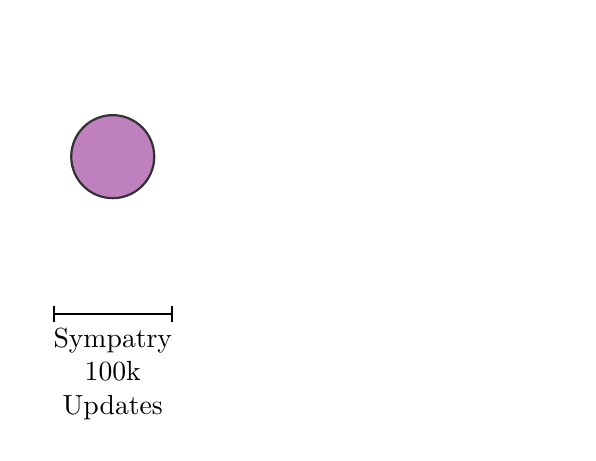
\begin{tikzpicture}
			\tikzstyle{main}=[circle, minimum size = 5mm, thick, draw =black!80, node distance = 10mm]
			\tikzstyle{connect}=[thick]
			\tikzstyle{box}=[rectangle, draw=black!100]
			\node[main, fill = violet!50] (a) [circle,minimum size=3em] {};
			\node[main, fill = red!50]                   (b) [semi,  minimum size=1.5em, shape border rotate=0, above right=0.7cm and 2cm of a, opacity=0] {};
			\node[main, fill = blue!50]                   (c) [semi,  minimum size=1.5em, shape border rotate=180, below right=0.7cm and 2cm of a, opacity=0] {};
			
			\node[main, fill = violet!50]                   (d) [circle,  minimum size=3em, shape border rotate=180, below right=0.7cm and 2cm of b, opacity=0] {};
			
		
			
			\draw [thick] (-0.75,-2) -- (0.75,-2) node [midway,below] {\begin{tabular}{c} Sympatry\\100k\\Updates\end{tabular}};
			\draw [thick] (-0.75,-1.9) -- (-0.75,-2.1);
			\draw [thick] (0.75,-1.9) -- (0.75,-2.1);

			
			
			
			\end{tikzpicture}
		\end{center}
	
%	\begin{enumerate}
%		\item Evolve in sympatry (single environment) for 100k updates.
%		\item Split into two separate populations (Allopatry) for 100k updates.
%		\item Rejoined for single round of mating.
%		\item 5 treatments with varying task sets during Sympatry and Allopatry, plus all-sympatric control.
%	\end{enumerate}	
%%%
% In order to study how sexual selection affects speciation, we set up evolving populations of sexual organisms, with sexes. The "female" chooses a "male" to mate with on the basis of a displayed trait.
%%%
% The populations are allowed to evolve in sympatry for a while, then the population is split in half, and each allowed to evolve independently. Finally, the halves are reunited for a single round of mating, and we measured the rate of hybridization.
}


\frame{
	\frametitle{Experimental Design}
	\begin{center}
		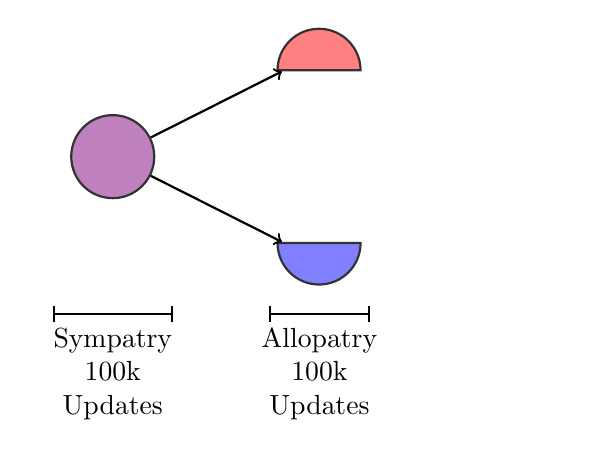
\begin{tikzpicture}
		\tikzstyle{main}=[circle, minimum size = 5mm, thick, draw =black!80, node distance = 10mm]
		\tikzstyle{connect}=[thick]
		\tikzstyle{box}=[rectangle, draw=black!100]
		\node[main, fill = violet!50] (a) [circle,minimum size=3em] {};
		\node[main, fill = red!50]                   (b) [semi,  minimum size=1.5em, shape border rotate=0, above right=0.7cm and 2cm of a] {};
		\node[main, fill = blue!50]                   (c) [semi,  minimum size=1.5em, shape border rotate=180, below right=0.7cm and 2cm of a] {};
		\node[main, fill = violet!50]                   (d) [circle,  minimum size=3em, shape border rotate=180, below right=0.7cm and 2cm of b, opacity=0] {};
		
		\path[->] 
		(a) edge [connect] (b)
		(a) edge [connect] (c)

		;
		
		\draw [thick] (-0.75,-2) -- (0.75,-2) node [midway,below] {\begin{tabular}{c} Sympatry\\100k\\Updates\end{tabular}};
		\draw [thick] (-0.75,-1.9) -- (-0.75,-2.1);
		\draw [thick] (0.75,-1.9) -- (0.75,-2.1);
		
		
		\draw [thick] (2,-2) -- (3.25,-2) node [midway,below] {\begin{tabular}{c} Allopatry\\100k\\Updates\end{tabular}};
		\draw [thick] (2,-1.9) -- (2,-2.1);
		\draw [thick] (3.25,-1.9) -- (3.25,-2.1);
		
		
		
		
		\end{tikzpicture}
	\end{center}
	
	%	\begin{enumerate}
	%		\item Evolve in sympatry (single environment) for 100k updates.
	%		\item Split into two separate populations (Allopatry) for 100k updates.
	%		\item Rejoined for single round of mating.
	%		\item 5 treatments with varying task sets during Sympatry and Allopatry, plus all-sympatric control.
	%	\end{enumerate}	
}

\frame{
	\frametitle{Experimental Design}
	\begin{center}
		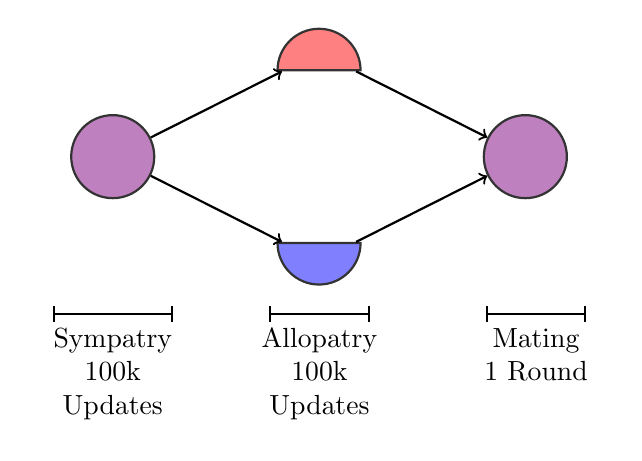
\begin{tikzpicture}
		\tikzstyle{main}=[circle, minimum size = 5mm, thick, draw =black!80, node distance = 10mm]
		\tikzstyle{connect}=[thick]
		\tikzstyle{box}=[rectangle, draw=black!100]
		\node[main, fill = violet!50] (a) [circle,minimum size=3em] {};
		\node[main, fill = red!50]                   (b) [semi,  minimum size=1.5em, shape border rotate=0, above right=0.7cm and 2cm of a] {};
		\node[main, fill = blue!50]                   (c) [semi,  minimum size=1.5em, shape border rotate=180, below right=0.7cm and 2cm of a] {};
		
		\node[main, fill = violet!50]                   (d) [circle,  minimum size=3em, shape border rotate=180, below right=0.7cm and 2cm of b] {};
		
		\path[->] 
		(a) edge [connect] (b)
		(a) edge [connect] (c)
		(b) edge [connect] (d)
		(c) edge [connect] (d)
		;
		
		\draw [thick] (-0.75,-2) -- (0.75,-2) node [midway,below] {\begin{tabular}{c} Sympatry\\100k\\Updates\end{tabular}};
		\draw [thick] (-0.75,-1.9) -- (-0.75,-2.1);
		\draw [thick] (0.75,-1.9) -- (0.75,-2.1);
		
		
		\draw [thick] (2,-2) -- (3.25,-2) node [midway,below] {\begin{tabular}{c} Allopatry\\100k\\Updates\end{tabular}};
		\draw [thick] (2,-1.9) -- (2,-2.1);
		\draw [thick] (3.25,-1.9) -- (3.25,-2.1);
		
		
		\draw [thick] (4.75,-2) -- (6,-2) node [midway,below] {\begin{tabular}{c} Mating\\1 Round\end{tabular}};
		\draw [thick] (4.75,-1.9) -- (4.75,-2.1);
		\draw [thick] (6,-1.9) -- (6,-2.1);
		
		% {l1} node[align=right, below]{Sympatry};
		
		
		\end{tikzpicture}
	\end{center}
	
	%	\begin{enumerate}
	%		\item Evolve in sympatry (single environment) for 100k updates.
	%		\item Split into two separate populations (Allopatry) for 100k updates.
	%		\item Rejoined for single round of mating.
	%		\item 5 treatments with varying task sets during Sympatry and Allopatry, plus all-sympatric control.
	%	\end{enumerate}	
}

\frame{
	\frametitle{Results - Pre-zygotic Isolation - Hybridization Rates Reduced}
	\begin{figure}[h!]
		\begin{center}
			\includegraphics[width=0.7\columnwidth]{figures/118_ratio_sum_matings_gen1__pretty_original.png}
		\end{center}
	\end{figure}
%%%
% We found that it works! In all treatments, we saw significantly reduced rates of hybridization between the split populations. This indicates a bit of pre-zygotic isolation.
}

\frame{
	\frametitle{Post-Zygotic Isolation - Viability of Offspring from Forced Matings}
	\begin{figure}[h!]
		\begin{center}
			\includegraphics[width=0.7\columnwidth]{figures/recombination_viability.png}
		\end{center}
	\end{figure}
%%%
% Interestingly, we also saw very little post-zygotic isolation in the form of reduced viability or fitness of hybrids. The effect was quite small, though it was significant. We would, however, expect this effect to be larger if we had let them evolve separately for longer.
}

\frame{
	\frametitle{Post-Zygotic Isolation - Fitness of Offspring from Forced Matings}
	\begin{figure}[h!]
		\begin{center}
			\includegraphics[width=0.7\columnwidth]{figures/recombination_fitness.png}
		\end{center}
	\end{figure}
}

\frame{
	\frametitle{Conclusion}
	\begin{enumerate}
		\item At short time-scales, Sexual Selection increases Pre-zygotic Isolation.
		\item Treatment environment was insufficient to create difference in effect.
	\end{enumerate}

}

%%%%%%%%%%%%%%%%%%%%%%%%%%%%%%%%%%%%%%%%%%%%%%%%%%%%%%%%%%%%%%%%%%%%%%%%%%%%%%

\section[Proposals]{Proposals}
%%%
% Now moving on to the proposals.	

\subsection[HGT]{Proposal: Horizontal Gene Transfer and Modularity}

\frame{
	\frametitle{Proposal: Horizontal Gene Transfer and Modularity}
	\begin{center}
		\includegraphics[width=0.7\columnwidth]{figures/Figure.png}
	\end{center}
%%%
% We want to study the effect that Horizontal Gene Transfer has on genetic architecture, and modularity in particular. 
% Horizontal gene transfer is any kind of transfer and homologous integration of genetic material that is not through vertical reproduction. This blanket term covers phenomena like plasmid transmission, natural competence, where you eat the dead for food and possibly incorporate bits of the genome, or viral infection. HGT occurs extremely frequently, particularly in Prokaryotes, but there is a bit of evidence of HGT in eukaryotes as well. 
}

\frame{
	\frametitle{Proposed Experiments}
	\begin{enumerate}
		\item Low Uptake Frequency: Static environment, Uptake Bonus vs No Bonus
		\item Higher Uptake Frequency: Changing environment, Uptake Bonus vs No Bonus
		\item Higher Fitnesses: Obligate HGT vs non-HGT
	\end{enumerate}
%%%
% We were interested in seeing under what circumstances HGT, natural competence in particular, would evolve, and what effect it would have on architecture and fitness.
% We think that in environments where evolvability is less imporant, organisms might use HGT, but only if there is a bonus associated to uptake.
% However, in environments with more pressure to evolve, we expect that organisms would uptake at a higher rate, for the chance to integrate useful function from the gene fragments floating around.
% Finally, we expect that obligate HGTers will have more modular genomes, and will have higher overall fitness, because of their faster adaptation.
}

%%%%%%%%%%%%%%%%%%%%%%%%%%%%%%%%%%%%%%%%%%%%%%%%%%%%%%%%%%%%%%%%%%%%%%%%%%%%%%
\subsection[Mutational Landscape]{Relating Robustness, Modularity and Evolvability with Mutational Neighborhood}

\frame{
	\frametitle{Relating Robustness, Modularity and Evolvability with Mutational Neighborhood}
		\begin{center}
			\includegraphics[width=0.45\columnwidth]{pictures/Col_de_Braus-small}
			\quad
			\includegraphics[width=0.45\columnwidth]{pictures/plateau.jpg}
		\end{center}
%%%
% The last proposal is a more open-ended project, where we want to look at the characteristics of mutational landscapes, and how those landscapes and where populations sit in them might mediate features like robustness and evolvability.		
}

%		\item Explore relationship between mutational landscape and measures of evolvability, modularity, and robustness.
%		\item Identify motifs of landscape shape that improve evolvability.
%		\item Determine whether mutational landscape network metrics are useful predictors of robustness, evolvability, and modularity.

\frame{
	\frametitle{Characterizing Mutational Landscapes via Network Graphs}
	\begin{center}
		\begin{tikzpicture}
		\tikzstyle{main}=[circle, minimum size = 5mm, thick, draw =black!80, node distance = 10mm]
		\tikzstyle{connect}=[thick]
		\tikzstyle{box}=[rectangle, draw=black!100]
		\node[main, fill = white!100] (a) [            label=275:$A$] { };
		\node[main]                   (b) [right=of a, label=275:$B$] {};
		\node[main]                   (c) [right=of b, label=275:$C$] {};
		\node[main]                   (d) [right=of c, label=275:$D$] {};
		\node[main]                   (e) [right=of d, label=275:$E$] {};
		
		\node[main, fill = red!50]    (f) [below=of b, opacity=0] {};	
		\node[main, fill = red!50]    (g) [below=of c, opacity=0] {};	
		\node[main, fill = black!100] (h) [below=of d, opacity=0] {};
		
		\node[main, fill = blue!50]   (i) [above=of b, opacity=0] {};
		\node[main, fill = orange!50] (j) [above=of c, opacity=0] {};
		\node[main, fill = black!100] (k) [above=of d, opacity=0] {};
		
		\path 
		(a) edge [connect] (b)
		
		(c) edge [connect] (d)
		
		(d) edge [connect] (e)
		
		;
		
		\end{tikzpicture}
	\end{center}
%%%
% To that end, we're developing a series of graph metrics to characterize populations in mutational landscape space.
% First, imagine that you have a population of organisms. You pick a phenotype in that population, and you enumerate all the unique genotypes in that phenotype.
% Then, you take those genotypes, and draw lines between them that are single-step mutations.
% The white nodes above are those genotypes.
}

\frame{
	\frametitle{Characterizing Mutational Landscapes via Network Graphs}
	\begin{center}
		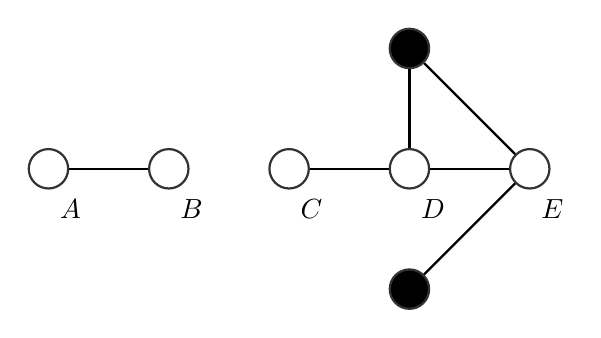
\begin{tikzpicture}
		\tikzstyle{main}=[circle, minimum size = 5mm, thick, draw =black!80, node distance = 10mm]
		\tikzstyle{connect}=[thick]
		\tikzstyle{box}=[rectangle, draw=black!100]
		\node[main, fill = white!100] (a) [            label=275:$A$] { };
		\node[main]                   (b) [right=of a, label=275:$B$] {};
		\node[main]                   (c) [right=of b, label=275:$C$] {};
		\node[main]                   (d) [right=of c, label=275:$D$] {};
		\node[main]                   (e) [right=of d, label=275:$E$] {};
		
		\node[main, fill = red!50]    (f) [below=of b, opacity=0] {};	
		\node[main, fill = red!50]    (g) [below=of c, opacity=0] {};	
		\node[main, fill = black!100] (h) [below=of d] {};
		
		\node[main, fill = blue!50]   (i) [above=of b, opacity=0] {};
		\node[main, fill = orange!50] (j) [above=of c, opacity=0] {};
		\node[main, fill = black!100] (k) [above=of d] {};
		
		\path 
		(a) edge [connect] (b)
		
		(c) edge [connect] (d)

		
		(d) edge [connect] (k)
		(d) edge [connect] (e)
		(e) edge [connect] (h)
		
		(e) edge [connect] (k)
		;
		
		\end{tikzpicture}
	\end{center}
%%%
% Then, you survey the 1-step mutational landscape surrounding each unique genotype. If you find a mutant that shares your phenotype, but doesn't exist, you add it to the graph, and mark it black. These are the unrealized genotypes in your phenotype, within 1 step of you. 
}



\frame{
	\frametitle{Characterizing Mutational Landscapes via Network Graphs}
	\begin{center}
		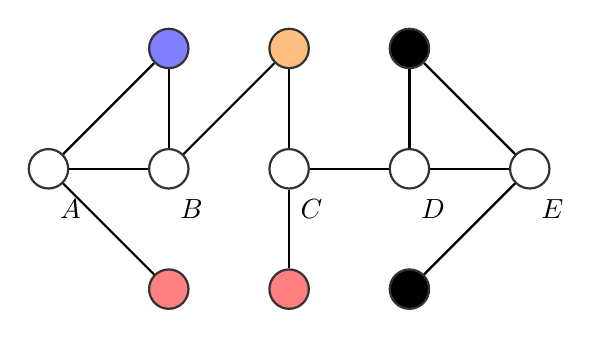
\begin{tikzpicture}
		\tikzstyle{main}=[circle, minimum size = 5mm, thick, draw =black!80, node distance = 10mm]
		\tikzstyle{connect}=[thick]
		\tikzstyle{box}=[rectangle, draw=black!100]
		\node[main, fill = white!100] (a) [            label=275:$A$] { };
		\node[main]                   (b) [right=of a, label=275:$B$] {};
		\node[main]                   (c) [right=of b, label=275:$C$] {};
		\node[main]                   (d) [right=of c, label=275:$D$] {};
		\node[main]                   (e) [right=of d, label=275:$E$] {};
		
		\node[main, fill = red!50]    (f) [below=of b] {};	
		\node[main, fill = red!50]    (g) [below=of c] {};	
		\node[main, fill = black!100] (h) [below=of d] {};
		
		\node[main, fill = blue!50]   (i) [above=of b] {};
		\node[main, fill = orange!50] (j) [above=of c] {};
		\node[main, fill = black!100] (k) [above=of d] {};
		
		\path 
		(a) edge [connect] (b)
		(a) edge [connect] (f)
		(a) edge [connect] (i)
		
		(b) edge [connect] (j)
		(j) edge [connect] (c)
		(b) edge [connect] (i)
		
		(c) edge [connect] (d)
		(c) edge [connect] (g)
		
		(d) edge [connect] (k)
		(d) edge [connect] (e)
		(e) edge [connect] (h)
		
		(e) edge [connect] (k)
		;
		
		\end{tikzpicture}
	\end{center}
%%%
% Finally, you add every other genotype you found in the 1-step space, and color them based on their phenotype.
% Using this kind of arrangement, we could potentially predict how robust a phenotype is, how evolvable it is, and so on.
}

\frame{
	\frametitle{Proposed Experiments}
	\begin{enumerate}
		\item Modularity Experiments: Asexual vs Sexual populations
		\item Robustness Experiment A: High Mutation Rate vs Normal Mutation rates
		\item Robustness Experiment B: Static Environments vs Changing Environments
	\end{enumerate}
%%%
% As part of exploring the potential of this approach, we want to examine the character of the mutational landscape under known conditions. For example, we would generate populations with high robustness and examine the mutational landscape that they inhabit.
% In this way, we might be able to predict what kinds of areas of the mutational landscape different kinds of populations occupy, and perhaps how better to guide the in certain directions.
}





%%%%%%%%%%%%%%%%%%%%%%%%%%%%%%%%%%%%%%%%%%%%%%%%%%%%%%%%%%%%%%%%%%%%%%
\section[Summary]{Summary}
\frame{
   \frametitle{Summary}
   \begin{enumerate}
  	   \item Evolvability is a complex, overlapping set of concepts.
	   \item Modularity and Robustness may either contribute to or diminish Evolvability depending on their context and scope.
	   \item Network measures for mutational landscapes may provide insights into how to produce more evolvable populations. 
   \end{enumerate}

}


%\section[]{Follow up}
%\frame{
%	\frametitle{There are some possible followup experiments.}
%	\begin{itemize}
%		\item todo
%		\pause
%		\item Remove synonymous mutations.
%		\pause
%		\item Look at more environments.
%		\pause
%		\item Add more degrees of freedom for biases to evolve.
%		\pause
%		\item Look at how mutation bias (doesn't?) change adaptation.
%	\end{itemize}
%}	

\frame{
	\frametitle{Thank you.}
	\begin{block}{Committee Members}
		\begin{tabular}{p{0.5\textwidth} p{0.5\textwidth}}
			Charles Ofria & Chris Adami\\
			Bill Punch & Fred Dyer
		\end{tabular}
	\end{block}
	
	\begin{block}{Collaborators}
			\begin{tabular}{p{0.5\textwidth} p{0.5\textwidth}}
				Charles Ofria & Mike Wiser\\
				Jason Keagy & 
			\end{tabular}
	\end{block}
	
	\begin{block}{DevoLab}
		\includegraphics[width=\textwidth]{pictures/devolab.png}
	\end{block}
}


%\frame{
%	\frametitle{Thank you.}
%	\begin{block}{Family \& Friends}
%	\begin{center}
	
%		\includegraphics[height=0.28\textwidth]{Images/JakeAndMe.png}
%		\includegraphics[height=0.28\textwidth]{Images/Family.png}\\
		
%		\includegraphics[height=0.28\textwidth]{Images/IMG_0051.png}
%		\includegraphics[height=0.28\textwidth]{Images/IMG_0056.png}
%	\end{center}
%\end{block}

%}

\begin{frame}[allowframebreaks]{References}
	\usebeamerfont{tiny}
	\bibliography{Comps,other_items}
\end{frame}



%\section[Future Work]{Future Work}
%\frame{
%	\frametitle{Future Work}
%	\begin{itemize}
%		\item Look at local landscaping to see the immediate effects of a mutation bias
%		\item Try competing instruction sets with evolved organisms
%		\item Introduce a different mutation bias in a small set of organisms during an experiment
%		\item Use the Path Finding environment
%	\end{itemize}
%}






%\frame{
%	MOAR STUFF.
%	}

%%%%%%%%%%%%%%%%%%%%%%%%%%%%%%%%%%%%%%%%%%%%%%%%%%%%%%%%%%%%%%
	% D R A G O N S    B E    H E R E
%%%%%%%%%%%%%%%%%%%%%%%%%%%%%%%%%%%%%%%%%%%%%%%%%%%%%%%%%%%%%%

\frame{
	\frametitle{Heritability and Response to Selection}
	\begin{block}{Fisher and Wright
			\cite{fisher_genetical_1930,wright_evolution_1931}
		}
		
		Narrow-sense Heritability
		\begin{equation}
		h^2 = \frac{Var_A}{Var_P}
		\end{equation}
		The Breeder's Equation
		\begin{equation}
		R = {h^2}S
		\end{equation}
	\end{block}
}

\frame{
	\frametitle{Measuring Spatial Modularity}
	\begin{quote}
		To measure Spatial Modularity, $m_S$:
		
		\begin{enumerate}
			\item count the total number of traits expressed in a genome: $T$
			\item identify the number of sites that code for any trait: set $K$
			\item count the number of items in set $K$: $k$
			\item count the number of traits coded for by each site within set $K$: $t_k$;
			\item calculate the inverse of the average number of traits coded for per site to reflect the level of spatial modularity ($m_S$) of coding regions of a genome
		\end{enumerate}
		\begin{equation}
		m_S = \frac{1}{\frac{1}{k} {\sum_{i=1}^{k} \frac{t_{k}}{T}}} 
		\end{equation}
	\end{quote}
}

\frame{
	\frametitle{Measuring Genotypic Robustness}
	
	\begin{quote}
		
		To measure Genotypic Robustness, $r_G$, of a genotype $G$:
		\begin{enumerate}
			\item count the number of loci in the genome: $n$
			\item count the number of possible alleles at a given site: $D$ 
			\item enumerate all possible single-step mutants that may arise from the given genotype (or sample from a more realistic distribution): $n(D-1)$;			
			\item count those mutants that prove to be neutral phenotypic variants: $R_G$;
			\item calculate the proportion of neutral phenotypic variants to reflect the probability of a neutral variant being produced by this genotype in response to mutation. 
			
		\end{enumerate}
		\begin{equation}
		r_{G} = \frac{R_{G}}{n(D-1)}
		\end{equation} 
	\end{quote}	
}

\frame{
	\frametitle{Measuring Phenotypic Robustness}
	\begin{quote}
		To measure Phenotypic robustness, $r_P$:
		
		\begin{enumerate}
			\item count the number of distinct neutral genetic variants that produce a given phenotypic trait in a population, ($Set K: k$);
			\item calculate the proportion of neutral variants produced by single-step mutations $r_G$, averaged over all of the neutral genetic variants to reflect the probability of a neutral genotype currently in the population producing another neutral genotype in response to mutation.
		\end{enumerate}
		\begin{equation}
		r_{P} = \frac{1}{k} \sum_{i=1}^{k} r_{G} 
		\end{equation}
	\end{quote}
}

\frame{
	\frametitle{Changing Environments - Experimental Details}
	\begin{enumerate}
		\item 150 Replicates, max 3600 individuals
		\item Fixed length organisms
		\item Cyclically changing environment, period of 1000 updates, equal-length phases.
		\item XOR task rewarded continuously
		\item EQU task rewarded/not rewarded according to cycle phase.
		\item Benign treatment - EQU not rewarded during off-cycle
		\item Hostile treatment - EQU punished during off-cycle
		\item Control treatment - No cycle, XOR and EQU always rewarded
	\end{enumerate}	
}

\frame{
	\frametitle{Changing Environments - Measurements}
	\begin{enumerate}
		\item Spatial Modularity of Last Common Ancestor (LCA) of Final Population  
		\item Population Phylogenetic Depth
		\item Population Per-Site and Average Genotypic Entropy 
		\item Per-site Task Performance along lineage of LCA.
		\item Proportion of sites related to Tasks
		\item Mutational Landscape
	\end{enumerate}	
}

\frame{
	\frametitle{Changing Environments - Results - Evolutionary History}
	\begin{figure}[h!]
		\begin{center}
			\includegraphics[width=0.45\columnwidth]{figures/flame_graph__control.png}
			\includegraphics[width=0.45\columnwidth]{figures/flame_graph__benign.png}\\
			\includegraphics[width=0.9\columnwidth]{figures/flame_graph__hostile.png}\\
			
		\end{center}
	\end{figure}
}

\frame{
	\frametitle{Changing Environments - Per-Site and Average Entropy - Control vs Benign}
	\begin{figure}[h!]
		\begin{center}
			\includegraphics[width=0.7\columnwidth]{figures/by_site_entropy__control.png}\\
			\includegraphics[width=0.7\columnwidth]{figures/by_site_entropy__benign.png}
			
		\end{center}
	\end{figure}
}

\frame{
	\frametitle{Changing Environments - Per-Site and Average Entropy - Control vs Hostile}
	\begin{figure}[h!]
		\begin{center}
			\includegraphics[width=0.7\columnwidth]{figures/by_site_entropy__control.png}\\
			\includegraphics[width=0.7\columnwidth]{figures/by_site_entropy__hostile.png}
			
		\end{center}
	\end{figure}
}
\frame{
	\frametitle{Changing Environments - Active and Vestigial Sites}
	\begin{figure}[h!]
		\begin{center}
			\includegraphics[width=0.7\columnwidth]{figures/site_count__functional.png}
			
			\vspace{0.5cm}
			
			\includegraphics[width=0.7\columnwidth]{figures/site_count__vestigial.png}
			
		\end{center}
	\end{figure}
}

\frame{
	\frametitle{Sexual Selection - Experimental Design - Treatment Task Sets}
	\usebeamerfont{small}\begin{figure}[h!]
		\begin{center}
			\begin{tabular}{|l|l|l|l|}
				\hline \textbf{Treatment} & \textbf{Sympatry Tasks} & \textbf{Allopatry Tasks 1} & \textbf{Allopatry Tasks 2} \\
				\hline Control & Logic 9 (all) & N/A & N/A \\
				
				\hline A (restricted) & Logic 9 (all) & \parbox[t]{2cm}{NOT, NAND, AND, ORN, OR, NOR, EQU} & \parbox[t]{2cm}{NOT, NAND, AND, ORN, ANDN, XOR, EQU} \\
				
				\hline B (expanded) & Logic 9 (all)  & \parbox[t]{2cm}{Logic 9 + 3AA, 3AB, 3AC, 3AD} & \parbox[t]{2cm}{Logic 9 + 3BA, 3BB, 3BC, 3BD} \\
				
				\hline C (expanded) & \parbox[t]{2cm}{NOT, NAND, AND, ORN} & \parbox[t]{2cm}{NOT, NAND, AND, OR, NOR, NOR, EQU} & \parbox[t]{2cm}{NOT, NAND, AND, ORN, ANDN, XOR, EQU} \\
				
				\hline D (drift) & Logic 9 (all) & Logic 9 (all) & Logic 9 (all) \\
				
				\hline E (expanded) & \parbox[t]{2cm}{Braided NOT, NAND, AND, ORN} & \parbox[t]{2cm}{NOT, NAND, AND, ORN, OR, NOR, EQU} & \parbox[t]{2cm}{NOT, NAND, AND, ORN, ANDN, XOR, EQU} \\ 
				\hline 
			\end{tabular}
		\end{center}
	\end{figure}
}

\frame{
	\frametitle{Sexual Selection - Measurements}
	\begin{enumerate}
		\item Hybridization Rates  
		\item Fitness and Viability of Forced-Mating Hybrids
	\end{enumerate}	
}

\frame{
	\frametitle{HGT - Hypotheses}
	\begin{enumerate}
		\item Organisms will uptake gene fragments if there is a reward bonus, despite risk of mutation.
		\item Organisms will uptake fragments in environments where evolvability is benificial, even without an energy bonus.
		\item Obligate HGTers will have more modular genomes.
		\item Obligate HGTers will have higher overall fitnesses, and better measures of evolvability.
	\end{enumerate}
}

\frame{
	\frametitle{Mutational Neighborhood - Measurements}
	\begin{enumerate}
		\item Neutral Network Density
		\item Network Evolvability, 
		\item Unrealized Network Robustness. 
		\item Spatial and Functional Modularity
		\item Genomic and Phenotypic Robustness
		\item Genomic Diffusion Rate
	\end{enumerate}
}

\frame{
	\frametitle{Mutational Landscape - Average Mutational Network Density}
	\begin{quote}
		
		To measure Average Network Density, $D_K$:
		
		\begin{enumerate}
			\item enumerate all white nodes (set $K$)
			\item count the proportion of edges to nodes within the phenotype (edges to other white nodes), for each white node in the graph ($\frac{D_k}{nm}$);
			\item calculate the average across all nodes in set $K$ to reflect the relatedness and clustering of the realized genomes in the phenotype.
		\end{enumerate}
		
		\begin{equation}
		D_{K} = {\frac{1}{k} \sum_{i=1}^{k}}\frac{D_k}{nm} 
		\end{equation}
		
	\end{quote}
}

\frame{
	\frametitle{Mutational Landscape - Unrealized Network Robustness}
	\begin{quote}
		
		To measure Unrealized Network Robustness, $U_K$:
		\begin{enumerate}
			\item enumerate all white nodes (set $K$)
			\item count the proportion of edges to potential mutants within the phenotype (edges to black nodes), for each white node in the graph ($\frac{U_k}{nm}$);
			\item calculate the average across all nodes in set $K$ to reflect the level of mutational robustness in the population for a given phenotype.
		\end{enumerate}
		
		\begin{equation}
		U_{K} = {\frac{1}{k} \sum_{i=1}^{k}}\frac{U_k}{nm} 
		\end{equation}
	\end{quote}
}

\frame{
	\frametitle{Mutational Landscape - Network Evolvability}
	\begin{quote}
		To measure Network Evolvability, $E_K$:
		\begin{enumerate}
			\item enumerate all white nodes (node $k$ in set $K$)
			\item from each node $k$, count the colored nodes($C$)
			\item for each $k$, calculate the entropy of the edges to colored nodes, to identify the diversity of phenotypes available from that node: $e_k$.
			\item normalize the entropy against the total number of colored node edges to reflect the probability of a genotype connecting to a variety of other phenotypes ($E_k=\frac{{e_{k}}*C}{nm}$).
			\item calculate the average across all nodes in set K to reflect the level of evolvability in the population for a given phenotype.
		\end{enumerate}
		\begin{equation}
		E_{K} = {\frac{1}{k} \sum_{i=1}^{k}} E_k 
		\end{equation}
		
	\end{quote}
	
}

\end{document}
